\documentclass[aspectratio=169,dvipsnames]{beamer}
\usepackage{graphicx}
\usepackage{tikz}
\usetikzlibrary{shapes,arrows,positioning}
\usepackage[export]{adjustbox}
\usepackage[brazil]{babel}
\usepackage{pgfplots}
\pgfplotsset{compat=1.8}
\usepackage{multicol}
\usepackage{siunitx}

\subtitle{Prof. Daniel C. Araújo}
\setbeamercolor{title page}{fg=RoyalBlue}
\setbeamercolor{date}{fg=OliveGreen}
\setbeamertemplate{title page}
{
  \vfill
  \begin{centering}
    {\usebeamerfont{title}\usebeamercolor[fg]{title}\inserttitle\par}
    \vskip0.25em%
    {\usebeamerfont{subtitle}\usebeamercolor[fg]{subtitle}\insertsubtitle\par}
    \vskip0.5em%
    %{\usebeamerfont{date}\usebeamercolor[fg]{date}\insertdate\par}
    \vfill
  \end{centering}
}


% Remove o rodapé
\setbeamertemplate{footline}{}

% Define o cabeçalho com os logos
\setbeamertemplate{headline}{
  \leavevmode%
  \begin{beamercolorbox}[wd=\paperwidth,ht=0.6cm,dp=0.5cm,right, colsep*=0pt]{section in head/foot}%
    
\includegraphics[height=0.8cm,valign=c]{Figs/Comum/unb.png} 
  \end{beamercolorbox}%
  \vskip0pt%
  \tikz \draw[thick] (0,0) -- (\paperwidth,0); % desenha a linha horizontal
}


\setbeamertemplate{footline}{
  \leavevmode%
    \tikz \draw[thick] (0,0) -- (\paperwidth,0);
  \hbox{%
  \begin{beamercolorbox}[wd=\paperwidth,ht=2.5ex,dp=3ex,center]{section in foot/foot}%
    Princípios de Comunicação para Engenharia
  \end{beamercolorbox}}%
  \vskip0pt%
}
% Remove os elementos padrão do cabeçalho
\date{\today}


\title{Ruído em Sistemas AM e FM}
%\subtitle{Princípios de Comunicação para Engenharia }
\author{Prof. Daniel C. Araújo}
\institute{Universidade de Brasília}
%\date{\today}

\begin{document}

\frame{\titlepage}


\section{Ruído em Sistemas de Banda-básica}


\begin{frame}{Análise de Ruído em Sistemas em Banda Base}
\begin{itemize}
    \item Sistemas em banda base são usados como referência para comparação de sistemas de modulação.
    \item O receptor consiste em um filtro passa-baixa ideal com largura de banda \( W \).
    \item Potência do ruído para entrada de ruído branco:
    \begin{equation*}
        P_{no} = \int_{-W}^{W} \frac{N_0}{2}df = N_0W
    \end{equation*}
    \item SNR em banda base:
    \begin{equation*}
        \frac{S}{N_b} = \frac{P_R}{N_0W}
    \end{equation*}
\end{itemize}
\end{frame}

\begin{frame}{Exemplo}

\begin{block} {Exercício}
    Encontre a SNR em um sistema em banda base com uma largura de banda de 5 kHz e com \(N_0 = 10^{-14} \text{W/Hz}\). A potência do transmissor é de 1 kilowatt e a atenuação do canal é \(10^{-12}\).
\end{block}
\end{frame}



\begin{frame}{Solução}
\begin{block}{ }

    Temos \(P_R = 10^{-12} P_T = 10^{-12} \times 10^3 = 10^{-9} \text{Watts}\). Portanto,
\begin{equation*}
\frac{S}{N_b} = \frac{P_R}{N_0W} = \frac{10^{-9}}{10^{-14} \times 5000} = 20.
\end{equation*}
Isso é equivalente a \(10 \log_{10} 20 = 13 \text{dB}\).
\end{block}
\end{frame}


\section{Ruído em modulação AM}

\begin{frame}{Demodulação para banda básica}

Considere o sinal recebido
$$
r(t) = Am(t)\cos(2\pi f_c t) + n(t).
$$

Na entrada do demodulador, é feito a multiplicação por um sinal oscilatório de mesma frequência $f_c$
\begin{align*}
r(t) \cos(2\pi f_c t + \phi) &= A_c m(t) \cos(2\pi f_c t) \cos(2\pi f_c t + \phi) + n(t) \cos(2\pi f_c t + \phi) \\
&= \frac{1}{2} A_c m(t) \cos(\phi) + \frac{1}{2} A_c m(t) \cos(4\pi f_c t + \phi) \\
&\quad + \frac{1}{2} [n_c(t) \cos(\phi) + n_s(t) \sin(\phi)] \\
&\quad + \frac{1}{2} [n_c(t) \cos(4\pi f_c t + \phi) - n_s(t) \sin(4\pi f_c t + \phi)]. 
\end{align*}
\end{frame}


\begin{frame}{Sinal de banda-básica}
    Após o filtro passa-baixa temos que:

    $$
y(t) = \frac{1}{2} A_c m(t) \cos(\phi) + \frac{1}{2} [n_c(t) \cos(\phi) + n_s(t) \sin(\phi)].
$$

Se o sinal estiver sincronizado, ou seja, $\phi = 0$

$$
y(t) = \frac{1}{2} A_c m(t)  + \frac{1}{2} n_c(t).
$$

\end{frame}


\begin{frame}{Cálculo da relação sinal ruído}
\begin{columns}[T]
\begin{column}{0.5\textwidth}
Determinação da potência "útil"
\begin{align*}
    P_u &= \frac{1}{4}\int _{-\infty}^{\infty} A^2_c m^2(t) dt\\ 
        &= \frac{1}{4} A^2_c P_m
\end{align*}
\end{column}

\begin{column}{0.5\textwidth}
Determinação da potência do ruído
\begin{align*}
    P_{n_c} &= \frac{1}{4}\textrm{E}\{ n^2_c(t)\} \\
            &=  \frac{1}{4} \int _{-W}^{W} \frac{N_0}{2} df \\
            &=  \frac{1}{4} 4W \frac{N_0}{2} \\
            &= \frac{N_0W}{2}
\end{align*}
\end{column}
\end{columns}
\end{frame}

\begin{frame}{Realação Sinal Ruído para o DSB-SC}
    \begin{block}{SNR}
    \begin{align*}
        \textrm{SNR} &= \frac{\frac{1}{4} A^2_c P_m}{ \frac{N_0W}{2}} \\
                     &=\frac{A^2_c P_m}{ 2N_0W} \\
                     &=\frac{P_r}{ N_0W} \\
                     &= \frac{S}{N_b}
    \end{align*} 
\end{block}
\end{frame}




\begin{frame}{Análise de sinal da modulação SSB}

 Considere o sinal recebido 

 \begin{align*}
r(t) &= A_c m(t) \cos(2\pi f_c t) + A_c m(t) \sin(2\pi f_c t) + n(t) \\
     &= (A_c m(t) + n_c(t)) \cos(2\pi f_c t) + (A_c m(t) - n_s(t)) \sin(2\pi f_c t).
\end{align*}

Após uso do filtro passa-baixa tem-se que

$$
y(t) = \frac{1}{2} A_c m(t)  + \frac{1}{2} n_c(t).
$$
    
\end{frame}


\begin{frame}{Cálculo da relação sinal ruído}
\begin{columns}[T]
\begin{column}{0.5\textwidth}
Determinação da potência "útil"
\begin{align*}
    P_u &= \frac{1}{4}\int _{-\infty}^{\infty} A^2_c m^2(t) dt\\ 
        &= \frac{1}{4} A^2_c P_m
\end{align*}
\end{column}

\begin{column}{0.5\textwidth}
Determinação da potência do ruído
\begin{align*}
    P_{n_c} &= \frac{1}{4}\textrm{E}\{ n^2_c(t)\} \\
            &=  \frac{1}{4} \int _{-W}^{W} \frac{N_0}{2} df \\
            &=  \frac{1}{4} 2W \frac{N_0}{2} \\
            &= N_0W
\end{align*}
\end{column}
\end{columns}
\end{frame}


\begin{frame}{Realação Sinal Ruído para o SSB}
    \begin{block}{SNR}
    \begin{align*}
        \textrm{SNR} &= \frac{\frac{1}{4} A^2_c P_m}{ \frac{N_0W}{4}} \\
                     &=\frac{A^2_c P_m}{ N_0W} \\
                     &=\frac{P_r}{ N_0W} \\
                     &= \frac{S}{N_b}
    \end{align*} 
\end{block}
\end{frame}


\begin{frame}{Ruído em modulação AM-Convencional}
    No sinal AM-convencional, sinal transmitido é dado por
    $$
    u(t) = A(1 + \alpha m_n(t) ) \cos (2\pi f_c t) 
    $$
    O sinal recebido é 
    $$
     r(t) = [A_c [1 + a_m(t)] + n_c(t)] \cos 2\pi f_c t - n_s(t) \sin 2\pi f_c t,
    $$

A componente DC na forma de onda demodulada é removido e, portanto, a saída do filtro passa-baixa é
    $$
    y(t) = \frac{1}{2} A_c a_m(t) + \frac{n_c(t)}{2}.
    $$
\end{frame}


\begin{frame}{Cálculo da relação sinal ruído}
\begin{columns}[T]
\begin{column}{0.5\textwidth}
Determinação da potência "útil"
\begin{align*}
  P_R = \frac{A_c^2}{2} [1 + \alpha ^2 P_{m}],
\end{align*}
\end{column}

\begin{column}{0.5\textwidth}
Determinação da potência do ruído
\begin{align*}
      P_{n_c} &= \frac{1}{4}\textrm{E}\{ n^2_c(t)\} \\
            &=  \frac{1}{4} \int _{-W}^{W} \frac{N_0}{2} df \\
            &=  \frac{1}{4} 4W \frac{N_0}{2} \\
            &= \frac{N_0W}{2}
\end{align*}
\end{column}
\end{columns}
\end{frame}



\begin{frame}{Relação Sinal Ruído para o AM-Convecional}
    \begin{block}{SNR}
        \begin{minipage}{0.48\linewidth}
            \begin{align*}
                \frac{S}{N}_{AM} &= \frac{1}{4} A_c^2 \alpha^2 P_{Mn} \\
                &= \frac{1}{4} \frac{A_c^2 \alpha^2 P_{Mn}}{P_{nc}} \\
                &= \frac{A_c^2 \alpha^2 P_{Mn}}{2N_0W} \\
            \end{align*}
        \end{minipage}
        \hfill
        \begin{minipage}{0.48\linewidth}
            \begin{align*}
                &= \frac{\frac{\alpha^2 P_{Mn}}{1 + \alpha^2 P_{Mn}} \frac{A_c^2}{2}}{N_0W} \\
                &= \frac{\alpha^2 P_{Mn}}{1 + \alpha^2 P_{Mn}} \frac{P_R}{N_0W} \\
                &= \frac{\alpha^2 P_{Mn}}{1 + \alpha^2 P_{Mn}} \frac{S}{N}_{b} \\
                &= \eta \left( \frac{S}{N} \right)_{b},
            \end{align*}
        \end{minipage}
    \end{block}
\end{frame}


\begin{frame}{Exemplo}
    \begin{block}{Comparação entre as modulações AM}
Assumimos que a mensagem é um processo aleatório estacionário em sentido amplo \( M(t) \) com a função de autocorrelação
\[ R_M(\tau) = 16 \text{sinc}^2(10,000\tau). \]

Também sabemos que todas as realizações do processo da mensagem satisfazem a condição
\[ \max |m(t)| = 6. \]

\end{block}
\end{frame}

\begin{frame}{Exemplo: Continuação}
\begin{block}{Continuação}
        Queremos transmitir essa mensagem para um destino através de um canal com atenuação de 50 dB e ruído aditivo branco com densidade espectral de potência \( S_N(f) = \frac{N_0}{2} = 10^{-12} \) W/Hz. Também queremos alcançar uma SNR na saída do modulador de pelo menos 50 dB. Qual é a potência do transmissor necessária e a largura de banda do canal se empregarmos os seguintes esquemas de modulação?

        \begin{itemize}
    \item DSB AM.
    \item SSB AM.
    \item AM convencional com índice de modulação igual a 0.8.
\end{itemize}

\end{block}

\end{frame}

\begin{frame}{Solução}
Primeiro, determinamos a largura de banda do processo da mensagem. Para fazer isso, obtemos a densidade espectral de potência do processo da mensagem, ou seja, $S_M(f) = g[R_M(\tau)] = \frac{16}{10,000} \Lambda \left( \frac{f}{10,000} \right)$, que é diferente de zero para \( -10,000 < f < 10,000 \); portanto, \( W = 10,000 \) Hz. Agora, podemos determinar \( \frac{S}{N}_b \) como uma base de comparação:
\[
\frac{S}{N}_b = \frac{P_R}{N_0W} = \frac{P_R}{2 \times 10^{-12} \times 10^4} = \frac{10^8 P_R}{2}.
\]

Uma vez que a atenuação do canal é de 50 dB, segue-se que $10 \log \frac{P_T}{P_R} = 50$
portanto,

\[
P_R = 10^{-5} P_T.
\]
\end{frame}

\begin{frame}{Solução: Continuação}
Assim,
\[
\frac{S}{N}_b = \frac{10^{-5} \times 10^8 P_T}{2} = \frac{10^3 P_T}{2}.
\]
1. Para DSB-SC AM, temos: $\frac{S}{N}_o = \frac{S}{N}_b = \frac{10^3 P_T}{2} \approx 50 \text{ dB} = 10^5.$

Portanto,
\[
\frac{10^3 P_T}{2} = 10^5 \implies P_T = 200 \text{ Watts}
\]
e
\[
BW = 2W = 2 \times 10,000 = 20,000 \text{ Hz} \approx 20 \text{ kHz}.
\]
\end{frame}

\begin{frame}{Solução: Continuação}
    2. Para SSB AM, temos:

\[
\frac{S}{N}_o = \frac{S}{N}_b = \frac{10^3 P_T}{2} = 10^5 \implies P_T = 200 \text{ Watts}
\]

e

\[
BW = W = 10,000 \text{ Hz} = 10 \text{ kHz}.
\]

\end{frame}


\begin{frame}{Solução: Continuação}
    3. Para AM convencional, com \( a = 0.8 \):

\[
\frac{S}{N}_o = \eta \frac{S}{N}_b = \eta \frac{10^3 P_T}{2}
\]

onde \( \eta \) é a eficiência de modulação dada por

\[
\eta = \frac{a^2 P_{Mn}}{1 + a^2 P_{Mn}}.
\]

Primeiro, encontramos \( P_{Mn} \), o conteúdo de potência do sinal de mensagem normalizado. Uma vez que \( \text{max} |m(t)| = 6 \), temos

\[
P_{Mn} = \frac{P_M}{(\text{max} |m(t)|)^2} = \frac{P_M}{36}.
\]

\end{frame}


\begin{frame}{Solução: Continuação}
Para determinar \( P_m \), temos:
\[ P_m = R_\eta (\tau)_{\tau=0} = 16; \]
Portanto,
\[ P_{mn} = \frac{16}{36} = \frac{4}{9}. \]
Assim,
\[ \eta = \frac{0.82 \times \frac{4}{9}}{1 + 0.82 \times \frac{4}{9}} \approx 0.22. \]
\end{frame}


\begin{frame}{Solução: Continuação}
Portanto,
\[ \frac{S}{N_0} \approx 0.22 \times \frac{10^3 P_T}{2} = 0.11 \times 10^3 P_T = 10^5 \]
ou
\[ P_T \approx 909 \text{ Watts}. \]
A largura de banda do AM convencional é igual à largura de banda do DSB AM, i.e.,
\[ BW = 2W = 20 \text{ kHz}. \]
\end{frame}



\section{Efeito do Ruído da Modulação Angular}

\begin{frame}{Modelo de sinal}
    \begin{align*}
u(t) &= A_c \cos(2\pi f_c t + \phi(t)) \\
     &= \left\{ 
         \begin{array}{ll}
         A_c \cos(2\pi f_c t + 2\pi k_f \int_{-\infty}^{t} m(\tau) d\tau) & \text{FM} \\
         A_c \cos(2\pi f_c t + k_p m(t)) & \text{PM}
         \end{array}
    \right.
\end{align*}
\begin{figure}
    \centering
    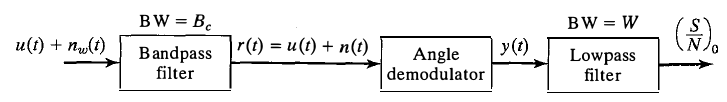
\includegraphics[width=0.85\linewidth]{Figs/FM/diagrama_bloco_fm.png}
    \caption{Diagrama de bloco do sistema FM}
    \label{fig:efm_ruido}
\end{figure}
\end{frame}


\begin{frame}{Modelo Vetorial}
    \begin{columns}[T] % O 'T' alinha o topo das colunas

    \begin{column}{0.5\textwidth} % Especifica que a coluna irá ocupar metade da largura do frame
        Considere o ruído de banda passante
        \begin{align*}
        n(t) &= \sqrt{n_c^2(t) + n_s^2(t)} \cos \left( 2\pi f_c t + \arctan \left( \frac{n_s(t)}{n_c(t)} \right) \right) \\
        &= V_n(t) \cos \left( 2\pi f_c t + \phi_n(t) \right),
        \end{align*}
        Vamos assumir que
        $$
        V_n(t) << A_c
        $$
    \end{column}

    \begin{column}{0.5\textwidth} % Especifica que a coluna irá ocupar metade da largura do frame
        \begin{figure}
            \centering
            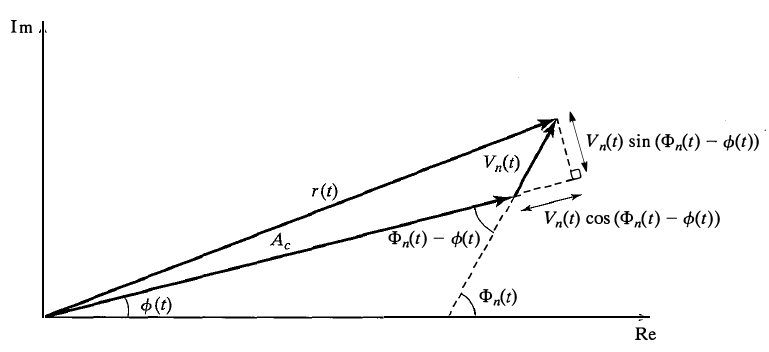
\includegraphics[width=0.8\linewidth]{Figs//FM/analise_vetorial.png}
            \caption{Representação Vetorial}
            \label{fig:enter-label}
        \end{figure}
    \end{column}

    \end{columns}
\end{frame}

\begin{frame}{Sinal recebido aproximado}
    \begin{align*}
r(t) &\approx (A_c + V_n(t) \cos(\phi_n(t) - \phi(t))) \\
&\quad \times \cos\left(2\pi f_c t + \phi(t) + \arctan\left(\frac{V_n(t) \sin(\phi_n(t) - \phi(t))}{A_c + V_n(t) \cos(\phi_n(t) - \phi(t))}\right)\right) \\
&\approx (A_c + V_n(t) \cos(\phi_n(t) - \phi(t))) \\
&\quad \times \cos\left(2\pi f_c t + \phi(t) + \frac{V_n(t) \sin(\phi_n(t) - \phi(t))}{A_c}\right) .
\end{align*}

\end{frame}


\begin{frame}{Sinal demodulado}
\begin{align*}
y(t) &= \left\{
\begin{array}{ll}
\phi(t) + \frac{V_n(t)}{A_c} \sin(\phi_n(t) - \phi(t)) & \text{PM} \\
\frac{1}{2\pi} \frac{d}{dt} \left( \phi(t) + \frac{V_n(t)}{A_c} \sin(\phi_n(t) - \phi(t)) \right) & \text{FM}
\end{array}
\right.
\\
&= \left\{
\begin{array}{ll}
k_{pm}(t) + \frac{V_n(t)}{A_c} \sin(\phi_n(t) - \phi(t)) & \text{PM} \\
k_{fm}(t) + \frac{1}{2\pi} \frac{d}{dt} \frac{V_n(t)}{A_c} \sin(\phi_n(t) - \phi(t)) & \text{FM}
\end{array}
\right.
\\
&= \left\{
\begin{array}{ll}
k_{pm}(t) + Y_n(t) & \text{PM} \\
k_{fm}(t) + \frac{1}{2\pi} \frac{d}{dt} Y_n(t) & \text{FM}
\end{array}
\right.
\end{align*}
Em que,
$Y_n(t) \equiv \frac{V_n(t)}{A_c} \sin\left(\phi_n(t) - \phi(t)\right) $
\end{frame}

%-----------------------------------------------------------------------------------------

\section{Lista de Exercícios}
\begin{frame}
  \frametitle{Exercício 1}

  \begin{block}{Questão}
    O sinal recebido $r(t) = s(t) + n(t)$ em um sistema de Comunicação
    passa por um filtro passa-baixa de largura de banda $W$ e ganho unitário.
    A componente $s(t)$ possui densidade espectral de potência
    $$
    S_s(f) = \frac{P_0}{1+\left(\frac{f}{B}\right)^2},
    $$
    em que $B$ é a banda de 3 dB. A componente de ruído possui densidade
    espectral de potência $\frac{N_0}{2}$ $\forall f$ $\in$ $\mathbb{R}$. Determine e
    faça o gráfico da SNR como uma função de $W/B$. Qual a largura de banda $W$ que 
    resultará na máxima $SNR$.
  \end{block}

\end{frame}

\begin{frame}
  \frametitle{Solução}

    O espectro do sinal na saída do filtro é
    $S_o(f) = S_s(f) |\Pi \left(\frac{f}{2W}\right)|^2$. Portanto, 
    a potência do sinal é 
    
    Se $W/B > 0$, a solução é:
    \begin{align*}
    \int_{-W}^{W} \frac{P_0}{1 + \left(\frac{f}{B}\right)^2} df &= P_0 B \left[\arctan\left(\frac{f}{B}\right)\right]_{-W}^{W} \\
    &= P_0 B \left(\arctan\left(\frac{W}{B}\right) - \arctan\left(-\frac{W}{B}\right)\right) \\
    &= P_0 B \cdot 2 \arctan\left(\frac{W}{B}\right)
    \end{align*}

    A potência do ruído na saída do filtro é $ P_{n,o} = \int _{-W}^{W} \frac{N_0}{2}df = N_0 W $

\end{frame}


\begin{frame}
  \frametitle{Solução}

  \begin{columns}
    \column{0.35\textwidth}
    \begin{align*}
      \text{SNR} &= \frac{P_0 B \cdot 2 \arctan\left(\frac{W}{B}\right)}{N_0 W} \\
      &= \frac{2P_0}{N_0} \frac{\arctan\left(\frac{W}{B}\right)}{\frac{W}{B}}
    \end{align*}
    \column{0.45\textwidth}
    \begin{figure}
      \centering 
  
      \begin{tikzpicture}
        \begin{axis}[
        domain=0.0001:10,
        xlabel=$\frac{W}{B}$,
        ylabel=$\frac{\arctan(\frac{W}{B})}{\frac{W}{B}}$,
        samples=100,
        smooth,
        scale=0.5,
        grid
        ]
        \addplot[blue,thick] {1/60*atan(x)/x};
        \end{axis}
      \end{tikzpicture}
  
  
    \end{figure}
    \end{columns}    
\end{frame}


\begin{frame}
  \frametitle{Questão 2}

  \begin{block}{Questão}
    Em um sistema de comunicação de radiodifusão, a 
    potência do transmissor é de 40 \si{\kilo\watt}, a atenuação do canal é de 80 dB e a
     potência de ruído é de $10^{-10}$ W/Hz.

     \begin{itemize}
      \item Encontre a SNR de pré-detecção.
      \item Encontre a SNR de saída se a modulação for DSB.
      \item Encontre a SNR de saída se a modulação for SSB.
      \item Encontre a SNR de saída se a modulação for AM convencional com um índice de modulação de 0,85 e possuir uma potência normalizada de mensagem de 0,2.
      \end{itemize}
  \end{block}

\end{frame}

\begin{frame}
  \frametitle{Solução}

  \begin{itemize}
    \item  Como a atenuação do canal é de 80 dB, então: 
    \begin{align*}
      P_R &= 10^{-8} \cdot P_T \\
        &= 10^{-8} \cdot 40 \cdot 10^3 \\
        & = 4 \cdot 10^{-4} \text{ Watts}
      \end{align*}
      Se o filtro limitador de ruído tem largura de banda B, então a potência de ruído pré-detecção é
      \begin{align*}
        P_n &= 2 \int_{f_c - B/2}^{f_c + B/2} \frac{N_0}{2}df = N_0B  \\
        & = 2 \times 10^{-10} B \text{Watts}.
      \end{align*}
    \item Portanto  : 
      \begin{equation*}
        SNR_{DSB,AM} = \frac{P_R}{P_n} = \frac{4\cdot 10^{-4}}{2 \cdot 10^{-10} \cdot 2 \cdot 10^4} = 100
        \end{equation*}
  \end{itemize}

\end{frame}

\begin{frame}
  \frametitle{Solução}
  \begin{itemize} 
    \item Para o caso SSB
  \begin{equation*}
    SNR_{SSB,AM} = \frac{P_R}{P_n} = \frac{4\cdot 10^{-4}}{2 \cdot 10^{-10} \cdot 10^4} = 200
    \end{equation*}
  
    \item $SNR_{DSB,o} = 2 SNR_{DSB,i} = 200 $
    \item $SNR_{SSB,o} = SNR_{SSB,i} = 200 $
    \item Sendo $\alpha = 0.8$ e $P_{M_n} = 0.2$ 
    \begin{equation}
      SNR_{AM,o} = \frac{\alpha^2 P_{M_n}}{1 + \alpha^2 P_{M_n}}SNR_{AM,i} = 0.1135 \cdot 2 \cdot 10^2
      \end{equation}
  \end{itemize}  

\end{frame}


\begin{frame}
  \frametitle{Questão 3}

  \begin{block}{Questão}
    Um canal de comunicação é caracterizado por uma atenuação de 90 dB e 
    por um ruído branco aditivo com densidade espectral de potência de 
    $0,5 x 10^{-14}$ W/Hz. A largura de banda da mensagem é de 1,5 MHz e 
    sua amplitude é uniformemente distribuída dentro do intervalo $[-1,1]$. 
    Se a SNR (razão sinal-ruído) necessária após a modulação é de 30 dB, 
    encontre a potência do transmissor em cada um dos casos.

    \begin{itemize}
      \item Modulação SSB.
      \item AM convencional com índice de modulação de 0,5 com potência normalizada 1/3.
      \item Modulação DSB-SC.
    \end{itemize}

  \end{block}

\end{frame}

\begin{frame}
  \frametitle{Solução}

  \begin{itemize}
    \item Primeiro passo é determinar a a SNR de banda-básica

    \begin{align*}
      \left(\frac{S}{N}\right) & = \frac{P_r}{N_0W} \\
      & = \frac{P_r}{2\cdot 0.5 \cdot 10^{-14} \cdot 1.5 \cdot 10^6} \\
      & = \frac{P_r10^8}{1.5}
    \end{align*}

    \item $P_r = 10^{-9}P_T$ 
    \item $\left(\frac{S}{N}\right) = \frac{P_r10^8}{1.5} = \frac{P_r}{15}$
  \end{itemize}

\end{frame}


\begin{frame}
  \frametitle{Solução}

  \begin{itemize}

    \item Portanto, a potência para o sistema SSB é

  \begin{align*}
    \left(\frac{S}{N}\right)_{SSB}  &= \left(\frac{S}{N}\right) = 10^3 \\
    P_T &= 15 \si{\kilo\watt}
  \end{align*}

  
    \item Para o caso AM-convencional tem-se que 
    \begin{align*}
      \left(\frac{S}{N}\right)_{AM-c} &= \frac{\alpha ^2 P_{M_n}}{1+\alpha ^2 P_{M_n}}\left(\frac{S}{N}\right) \\
      &=\frac{0.25 \cdot \frac{1}{3}}{1 + 0.25 \cdot \frac{1}{3}} \frac{P_T}{15} \\
      P_T& =195 \si{\kilo\watt}
    \end{align*}
  \end{itemize}
 
\end{frame}


\begin{frame}
  \frametitle{Solução}

  \begin{itemize}
    \item Similarmente ao caso SSB, tem-se que 
    \begin{align*}
      \left(\frac{S}{N}\right)_{SSB}  &= \left(\frac{S}{N}\right) = 10^3 \\
      P_T &= 15\si{\kilo\watt}
    \end{align*} 
  \end{itemize}  

\end{frame}





\begin{frame}
  \frametitle{Questão 4}

  \begin{block}{Questão}
    O sinal de mensagem normalizado $m_n(t)$ tem uma largura de banda de 
    5 \si{\kilo \hertz} e uma potência de 0.1 \si{\watt}. O canal tem uma largura 
    de banda de 100 \si{\kilo \hertz} e uma atenuação em 80 dB. O ruído é branco com
    uma densidade espectral de potência $0,5 \times 10^{-12}$ \si{\watt \per \hertz} e a potência do transmissor é 
    10 \si{\kilo \watt}.  

    \begin{itemize}
      \item Se AM com índice de modulação $\alpha = 0.8$ , qual é  SNR de saída?
      \item Se FM é empregado, qual é a SNR mais alta possível?
    \end{itemize}

  \end{block}
  
\end{frame}


\begin{frame}
  \frametitle{Solução do item 1}
   A potência do sinal recebido pode ser encontrada como: 

  \begin{align*}
  10\log{\frac{P_T}{P_R}} &= 80\\
  P_R &= 10^{-8}P_T\\
  P_R &= 10^{-4} W 
  \end{align*}
  
  
  \begin{align*}
  \left(\frac{S}{N}\right)_o &= \frac{ \alpha^2 P_{Mn}}{1 + \alpha^2 P_{Mn}} \left(\frac{S}{N}\right)_b
  &= \frac{ \alpha^2 P_{Mn}}{1 + \alpha^2 P_{Mn}} \frac{P_R}{N_0W}
  \end{align*}
  

  Assim, com $P_R = 10^{-4}$, $P_{Mn} = 0.1$, $\alpha = 0.8$ e $$N_0W = 2 \times 0.5 \times 10^{-12} \times 5 \times 10^3 = 5 \times 10^{-9}$$
\vspace*{-1cm}

$$ \left(\frac{S}{N}\right)_o = 1204 \approx 30.806 dB $$

\end{frame}

\begin{frame}
  \frametitle{Solução do item 2}

  2. Usando a Regra de Carson, nós obtemos: 

\begin{align*}
B_c &= 2(\beta+1)W \\
100 \times 10^3 &= 2(\beta+1)5 \times 10^3 \\
\beta &= 9
\end{align*}

Verificamos agora se o limite impõe alguma restrição. 

\begin{align*}
\left(\frac{S}{N}\right)_{b,th} & = 20(\beta +1)\\
20000&= 20(\beta +1)\\
\beta &= 999
\end{align*} 

\end{frame}

\begin{frame}
  \frametitle{Solução do item 2}

  Como estamos limitados em largura de banda, escolhemos $\beta = 9$. *A relação sinal/ruído de saída é: 

\begin{align*}
\left(\frac{S}{N}\right)_{o} &= 3\beta^20.1\left(\frac{S}{N}\right)_{b}\\
&= 3 \times 9^2 \times0.1 \times \frac{10^5}{5}\\
&= 48600 \approx 56.866 db
\end{align*}

\end{frame}



\begin{frame}
  \frametitle{Questão 5}
\scriptsize
  \begin{block}{Questão}
    Um sinal de mensagem normalizado tem uma largura de banda de $W = 8 \si{\kilo \hertz}$
     e uma potência de $P_{Mn} = \frac{1}{2}$. É necessário transmitir este sinal 
     através de um canal com largura de banda disponível de 60 KHz e atenuação de 40 \si{\decibel}.
     O ruído do canal é aditivo e branco com uma densidade espectral de potência de 
     $\frac{N_0}{2} = 10^{-12}$ \si{\watt \per \hertz}. Um esquema de modulação de frequência, 
     sem filtragem de pré-ênfase/de-ênfase, foi proposto para esse fim.

     \begin{enumerate}
      \item Se for desejável ter um SNR de pelo menos 40 \si{\decibel} na saída do receptor, qual é a potência mínima necessária do transmissor e o índice de modulação correspondente?
      \item Se a SNR mínima exigida for aumentada para 60 \si{\decibel}, como sua resposta mudaria?
      \item Se na parte 2 pudermos empregar filtros de pré-ênfase/de-ênfase com uma constante de tempo de $\tau = 75 \si{\micro \second} $ , como a resposta da parte 2 mudaria?
    \end{enumerate}
    
  \end{block}

\end{frame}




\begin{frame}
  \frametitle{Solução do item 1}
  Primeiro, verificamos se o limite ou a largura de banda impõem um limite restritivo no índice de modulação. Pela regra de Carson temos:

\begin{align*}
B_c &= 2(\beta+1)W \\
60 \times 10^3 &= 2(\beta+1) 8 \times 10^3 \\
\beta &= 2.75
\end{align*}

Usando a relação $$\left(\frac{S}{N}\right)_o = 60 \beta^2(\beta+1)P_{Mn}$$


\end{frame}


\begin{frame}
  \frametitle{Solução do item 1}

  Com $ \left(\frac{S}{N}\right)_o = 10^4$ e $P_{Mn} = \frac{1}{2}$ nos encontramos: 

$$10^4 = 30 \beta^2(\beta+1)$$
$$\beta = 6.6158$$

Como estamos limitados em largura de banda, escolhemos $\beta = 2,75$. Então,

\begin{align*}
\left(\frac{S}{N}\right)_o &= 3\beta^2P_{Mn}\left(\frac{S}{N}\right)_b\\
\left(\frac{S}{N}\right)_b &= \frac{2 \times 10^4}{3 \times 2.75^2} \\
&= 881.542
\end{align*}


\end{frame}


\begin{frame}
  \frametitle{Solução do item 1}

  Assim, 

\begin{align*}
\left(\frac{S}{N}\right)_b &= \frac{P_R}{N_0W} = 881.542\\
P_R &= 881.542 \times 2 \times 10^{-12} \times 8 \times 10^3 \\
P_R &= 1.41 \times 10^{-5}
\end{align*}

omo a atenuação do canal é de 40 db, encontramos: 

$$P_T = 10^4P_R = 0.141 W$$


\end{frame}

\begin{frame}
  \frametitle{Solução do item 2}

  Se a SNR mínima exigida for aumentada para 60 db, então o $\beta$ da regra de Carson permanece o
mesmo, enquanto a partir da relação

$$\left(\frac{S}{N}\right)_o = 60 \beta^2(\beta+1)P_{Mn}= 10^6$$

Encontramos $\beta = 31,8531$. Como na parte 1), escolhemos $\beta = 2,75$ e, portanto,

\begin{align*}
\left(\frac{S}{N}\right)_b &= \frac{1}{3\beta^2P_{Mn}}\left(\frac{S}{N}\right)_o = 8.8154 \times 10^4
\end{align*}

\end{frame}


\begin{frame}
  \frametitle{Solução item 2}

  Assim, 

\begin{align*}
  P_R &= N_0W \times 8.8154 \times 10^4 \\
     &= 2 \times 10^{-12} \times 8 \times 10^3 \times 8.8154 \times 10^4 \\
     &= 0.0014
\end{align*}

e

$$P_T = 10^4 P_R = 14 W$$

\end{frame}


\begin{frame}
  \frametitle{Solução item 3}

  A resposta de frequência do filtro do receptor (de-ênfase) é dada por: 


$$H_d(f) = \frac{1}{1+j \frac{f}{f_0}}$$

Como $f_0 = \frac{1}{2 \pi \times 75 \times 10^{-6}} = 2100Hz$. Neste caso: 

\begin{align*}
\left(\frac{S}{N}\right){o,PD} =  \frac{\left(\frac{W}{f_0} \right)^3}{3 \left( \frac{W}{f_0} - arctan \frac{W}{f_0} \right)} \left(\frac{S}{N}\right){o} = 10^6 
\end{align*}



\end{frame}

\begin{frame}
  Assim temos 

$$
\left(\frac{S}{N}\right)_{o} = \frac{10^6}{\left( \frac{\left(\frac{8 \cdot 10^3}{2100}\right)^3}{3 \cdot\left(\frac{8 \cdot 10^3}{2100}-\arctan \left(\frac{8 \cdot 10^3}{2100}\right)\right)} \right)} = 1.3541 \times 10^5
$$


Com isso encontramos: 


$$ P_R = 9.55 \times 10^{-5}$$


e, portanto, 

$$P_T = 10^4P_R = 0.955W$$

\end{frame}

\section{Figura de Ruído}





\begin{frame}
  \frametitle{Questão 6}


  \begin{block}{Questão}
    Um amplificador possui largura de banda equivalente de 25 \si{\kilo\hertz} e ganho de 30 \si{\decibel}. A potência na saída é 
    de $10^8 k T_0$, em que $T_0$  define a temperatura ambiente. Determine a temperatura efetiva de ruído e a
    figura de ruído.
  \end{block}
  

\end{frame}








\begin{frame}
  \frametitle{Solução}

    Considere  que 

$$
P_{n_0} = GK B_{neq} (T + T_e)
$$
Substituindo os valores tem-se Questão
\begin{align*}
  P_{n_0} &= GK B_{neq} (T + T_e) \\
  10^8 k T_0&= 10^{3} \cdot k \cdot 25 \times 10^{3} (T_0 + T_e) \\
  T_e &= \frac{10^8 - 25 \times 10^{6}}{ 25 \times 10^{6}}T_0  \\
  &= \frac{75 \times 10^{6}}{ 25 \times 10^{6}}T_0  \\
  &= 3T_0  \\
\end{align*}
\end{frame}

\begin{frame}
  \frametitle{Solução}

  Portanto a figura de ruído é
$$
F = \left(1 + \frac{3T_0}{T_0}\right) = 4
$$ 

\end{frame}

\end{document}